% !TeX encoding = UTF-8
\documentclass[aspectratio=169]{beamer}
\useoutertheme[progressbar=frametitle]{metropolis}
\useinnertheme{metropolis}
\definecolor{nabgray}{rgb}{0.6,0.59,0.61}
\usecolortheme[named=nabgray]{structure}

\usepackage{tikz}
\usepackage[utf8]{inputenc}
\usepackage[portuguese]{babel}
\usepackage{fontspec}
\setmonofont{JetBrains Mono}
\setmainfont{Roboto}
\setsansfont{Roboto}

\usepackage{smartdiagram}
\usepackage{qtree}
\usepackage[edges]{forest}
\usepackage{verbatim}
\usepackage{svg}
\usepackage{graphicx}
\usepackage{color}


\definecolor{lightgray}{rgb}{0.95, 0.95, 0.95}
\definecolor{darkgray}{rgb}{0.4, 0.4, 0.4}
%\definecolor{purple}{rgb}{0.65, 0.12, 0.82}
\definecolor{editorGray}{rgb}{0.95, 0.95, 0.95}
\definecolor{editorOcher}{rgb}{1, 0.5, 0} % #FF7F00 -> rgb(239, 169, 0)
\definecolor{editorGreen}{rgb}{0, 0.5, 0} % #007C00 -> rgb(0, 124, 0)
\definecolor{orange}{rgb}{1,0.45,0.13}
\definecolor{olive}{rgb}{0.17,0.59,0.20}
\definecolor{brown}{rgb}{0.69,0.31,0.31}
\definecolor{purple}{rgb}{0.38,0.18,0.81}
\definecolor{lightblue}{rgb}{0.1,0.57,0.7}
\definecolor{lightred}{rgb}{1,0.4,0.5}
\definecolor{ocherCode}{rgb}{1, 0.5, 0} % #FF7F00 -> rgb(239, 169, 0)
\definecolor{blueCode}{rgb}{0, 0, 0.93} % #0000EE -> rgb(0, 0, 238)
\definecolor{greenCode}{rgb}{0, 0.6, 0} % #009900 -> rgb(0, 153, 0)


\usepackage{upquote}
\usepackage{listings}
\lstset{language=java,
    otherkeywords={var,record},
    % Basic design
    backgroundcolor=\color{lightgray},
    basicstyle={\small\ttfamily},
    frame=l,
    keywordstyle=\footnotesize\color{blue},
    escapeinside={<@}{@>},
    breaklines=true,
    % Line numbers
    xleftmargin={0.75cm},
    numbers=left,
    stepnumber=1,
    firstnumber=1,
    numberfirstline=true
    % Code design
    identifierstyle=\color{black},
    keywordstyle=\color{ocherCode}\bfseries,
    ndkeywordstyle=\color{greenCode}\bfseries,
    stringstyle=\color{ocherCode}\ttfamily,
    commentstyle=\color{darkgray}\ttfamily,
    tabsize=2,
    showtabs=true,
    showspaces=false,
    showstringspaces=false,
    extendedchars=true,
    breaklines=true
}

\lstdefinelanguage{bash}{
    basicstyle=\ttfamily,
    showstringspaces=false,
    commentstyle=\color{red},
    keywordstyle=\color{blue},
    numbers=right,
    xleftmargin={0.25cm}
}


\usebackgroundtemplate%
{%
    
\includegraphics[width=\paperwidth]{Images/Contenido}%
}

\title{MicroProfile Benefits for Monolithic Applications}
\author{Víctor Orozco}
\institute{@tuxtor}
\date{\today}

\begin{document}

\frame{\titlepage}

\section{Modular monoliths}



\begin{frame}{Todo mundo odeia os monólitos . . . so que não}

\begin{columns}
\begin{column}{0.5\textwidth}
	\begin{figure}
		\centering
		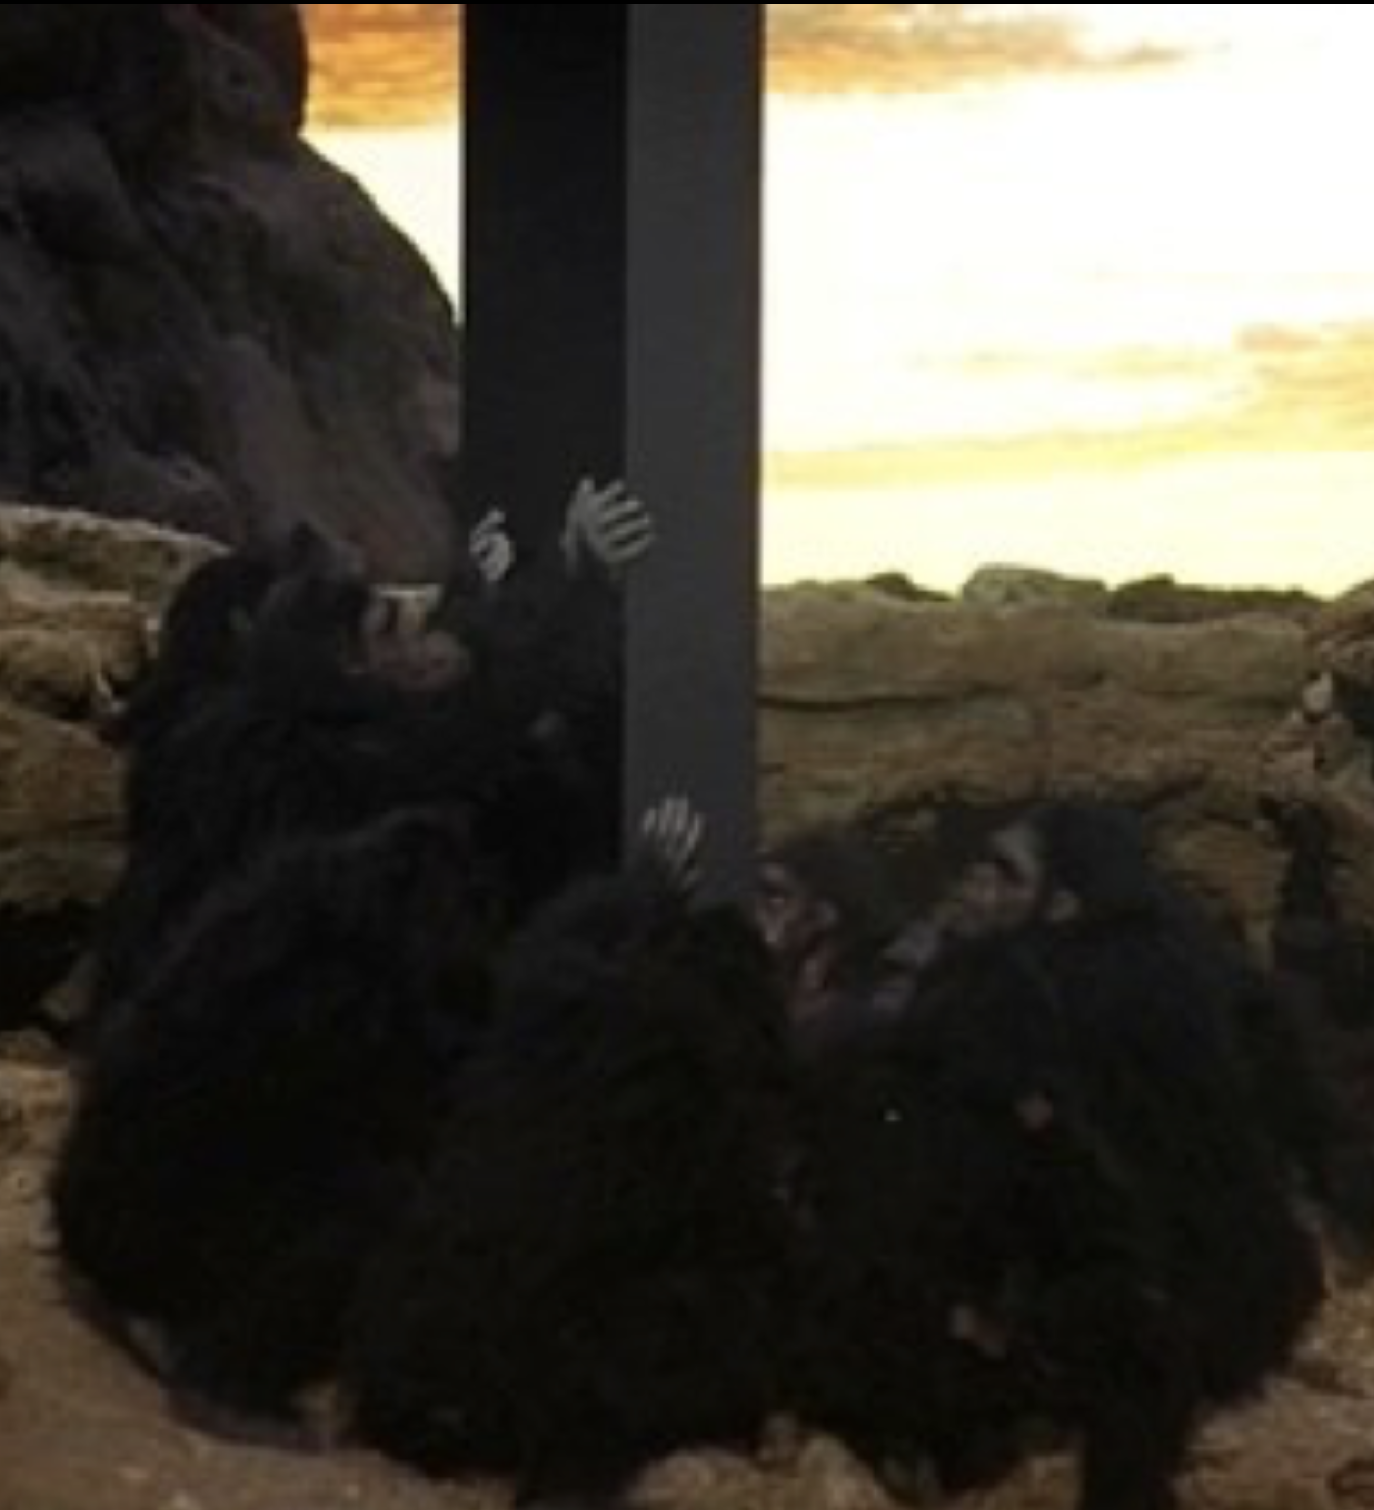
\includegraphics[width=0.7\linewidth]{Images/space}
	\end{figure}
	\end{column}
	\begin{column}{0.5\textwidth}  %%<--- here
		\begin{itemize}
        	\item Java vem criando sistemas "legados" desde 1995
            \item O mundo ainda tenta sair do Java 8
            \item Banca, governo, telco
            \item Nem todo mundo é Netflix
        \end{itemize}
	\end{column}
\end{columns}


\end{frame}

\begin{frame}{Java no mundo real}
"Como consultor independente é difícil aceitar que muito do trabalho real é garantir a continuidade para sistemas legados"\\

{\scriptsize Eu, bem triste mas com dinheiro na bolsa}
\end{frame}


\begin{frame}{2020 o ano da gurmetização do monólito}
\begin{figure}
	\centering
	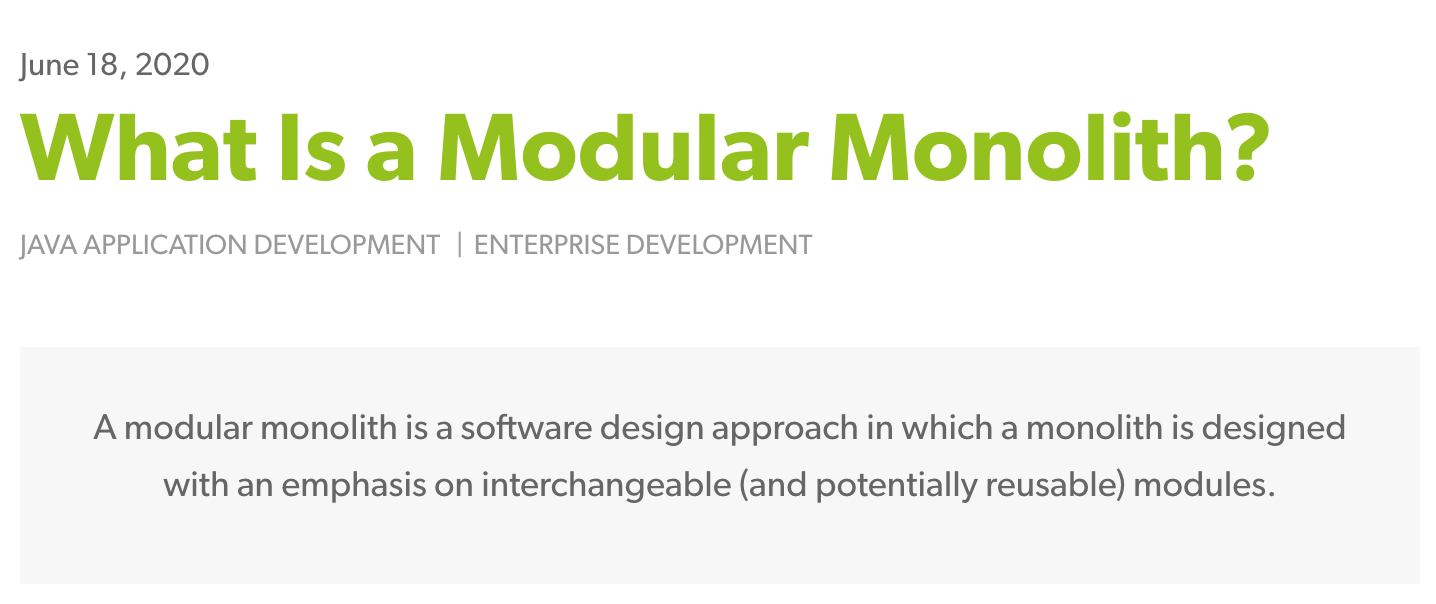
\includegraphics[width=0.8\linewidth]{Images/mmonolith1}
	\caption{JRebel}
\end{figure}
\end{frame}

\begin{frame}{2020 o ano da gurmetização do monólito}
\begin{figure}
	\centering
	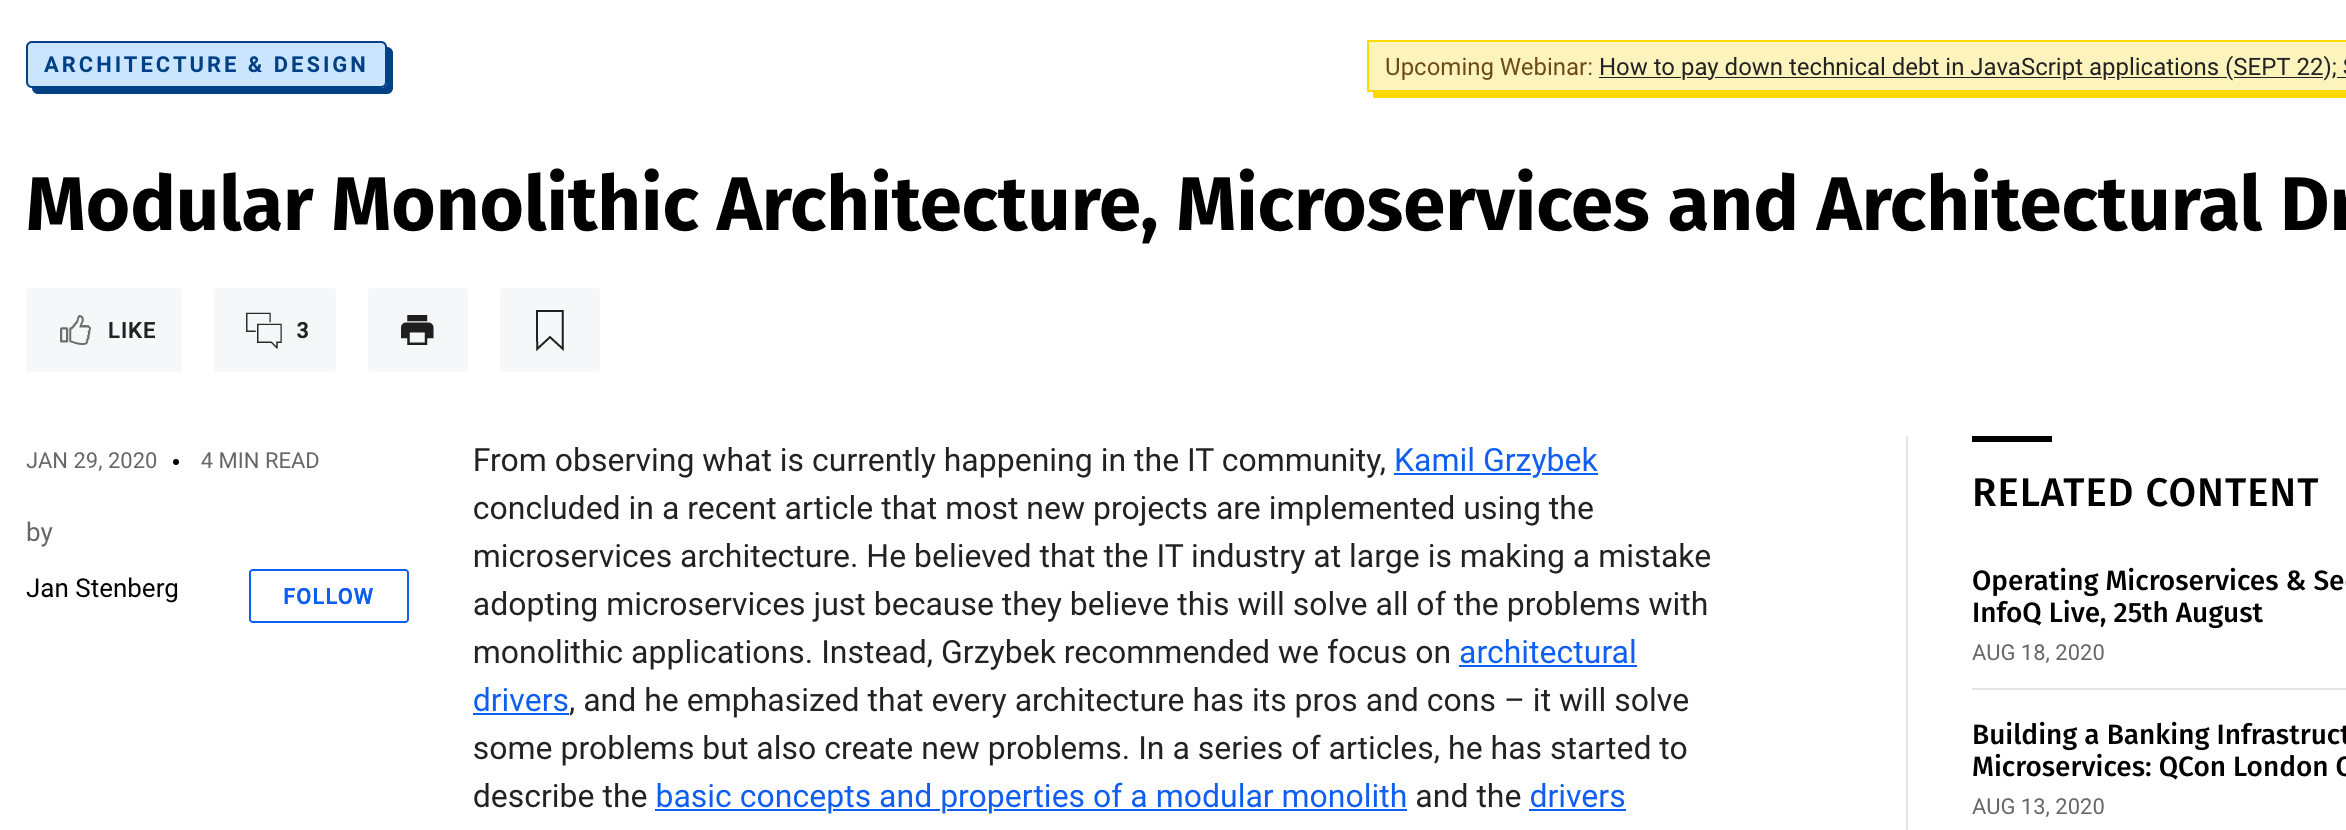
\includegraphics[width=0.8\linewidth]{Images/mmonolith2}
	\caption{InfoQ}
\end{figure}
\end{frame}


\begin{frame}{Microserviços}
Vantagens: Elasticidade, tolerância à falhas, responsividade
\begin{figure}
\centering
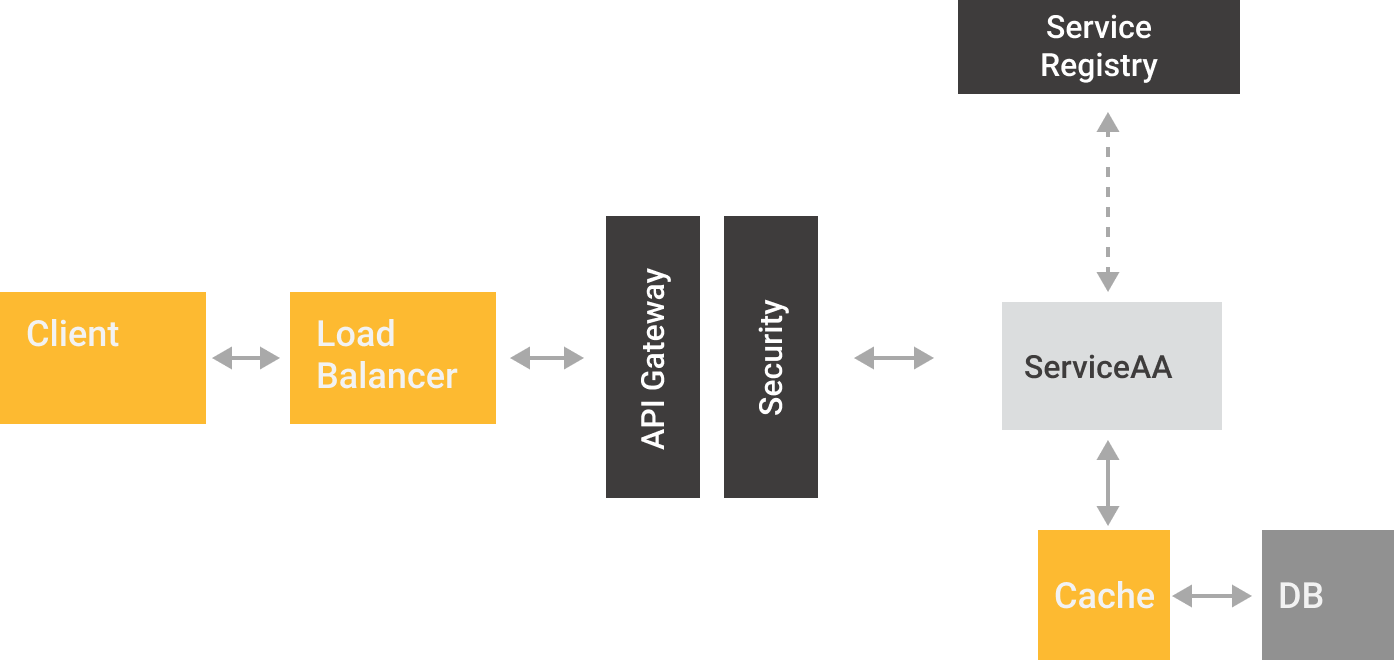
\includegraphics[width=0.7\linewidth]{Images/microservicios}
\caption{Microservicios}
\end{figure}
Desvantagens: Complexidade de desenvolvimento, integração é gestão
\end{frame}


\begin{frame}{Modular monolith}

    \begin{columns}
        \begin{column}{0.5\textwidth}
    	   O objetivo nunca foi criar um exercito de mini aplicativos. O objetivo sempre foi criar "reactive apps" ou seja aplicativos responsivos e escaláveis.
    	\end{column}
    	\begin{column}{0.5\textwidth}  %%<--- here
        Modular monolith = Monólito criado de forma modular
    		\begin{enumerate}
                \item Módulos intercambiáveis
                \item Funcionalidade autônoma para cada modulo
                \item Encapsulação garantida por contratos/interfaces
            \end{enumerate}

    	\end{column}
    \end{columns}
            \url{https://www.kamilgrzybek.com/design/modular-monolith-primer/}
\end{frame}


\begin{frame}{Modular monolith}
Modular monolith = SOA modular sem XML
\begin{figure}
	\centering
	
\includegraphics[width=\linewidth]{Images/cat}
\end{figure}

\end{frame}

\section{Eclipse MicroProfile}

\begin{frame}{Jakarta EE}
\begin{figure}
	\centering
	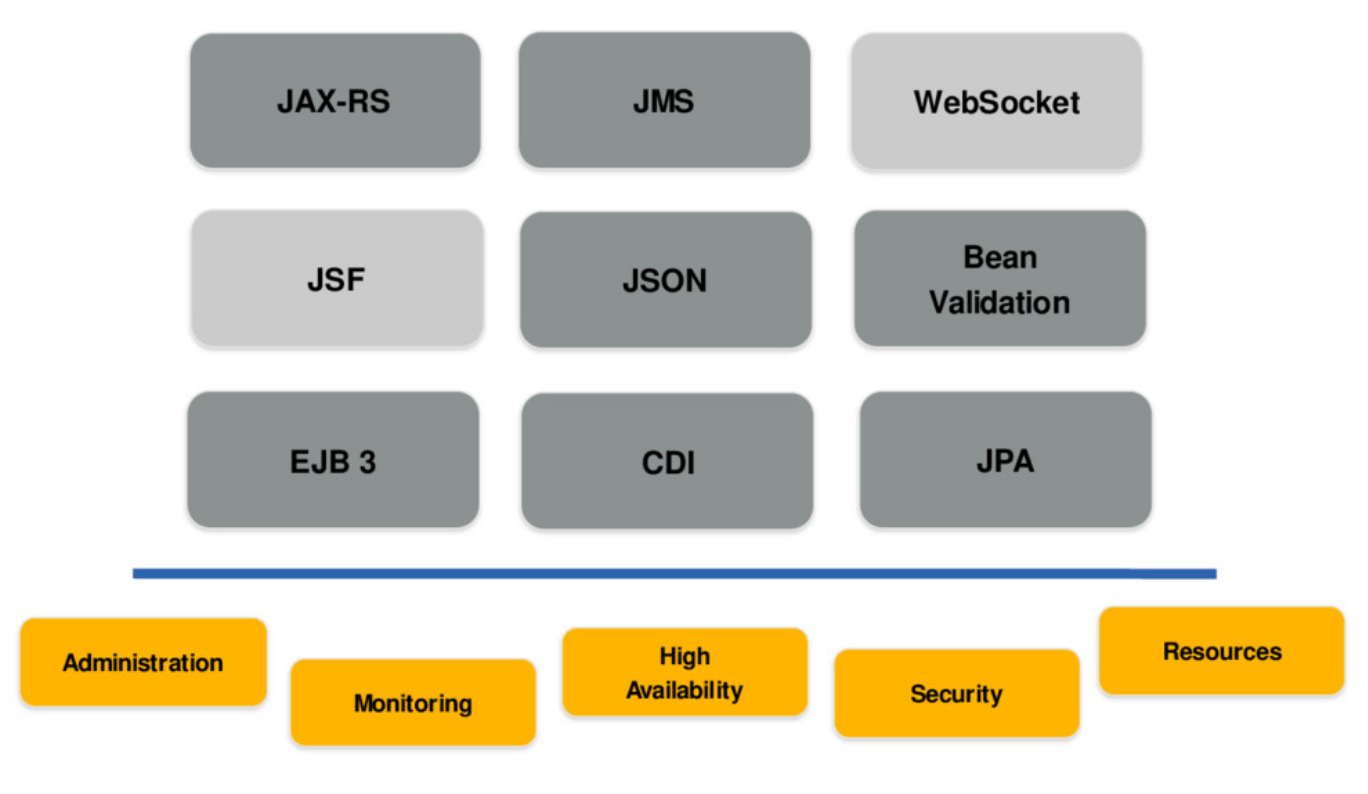
\includegraphics[width=0.8\linewidth]{Images/javaeemicropancake}
	\caption{Credito: Reza Rahman}
\end{figure}
\end{frame}


\begin{frame}{Eclipse MicroProfile}
\begin{figure}
	\centering
	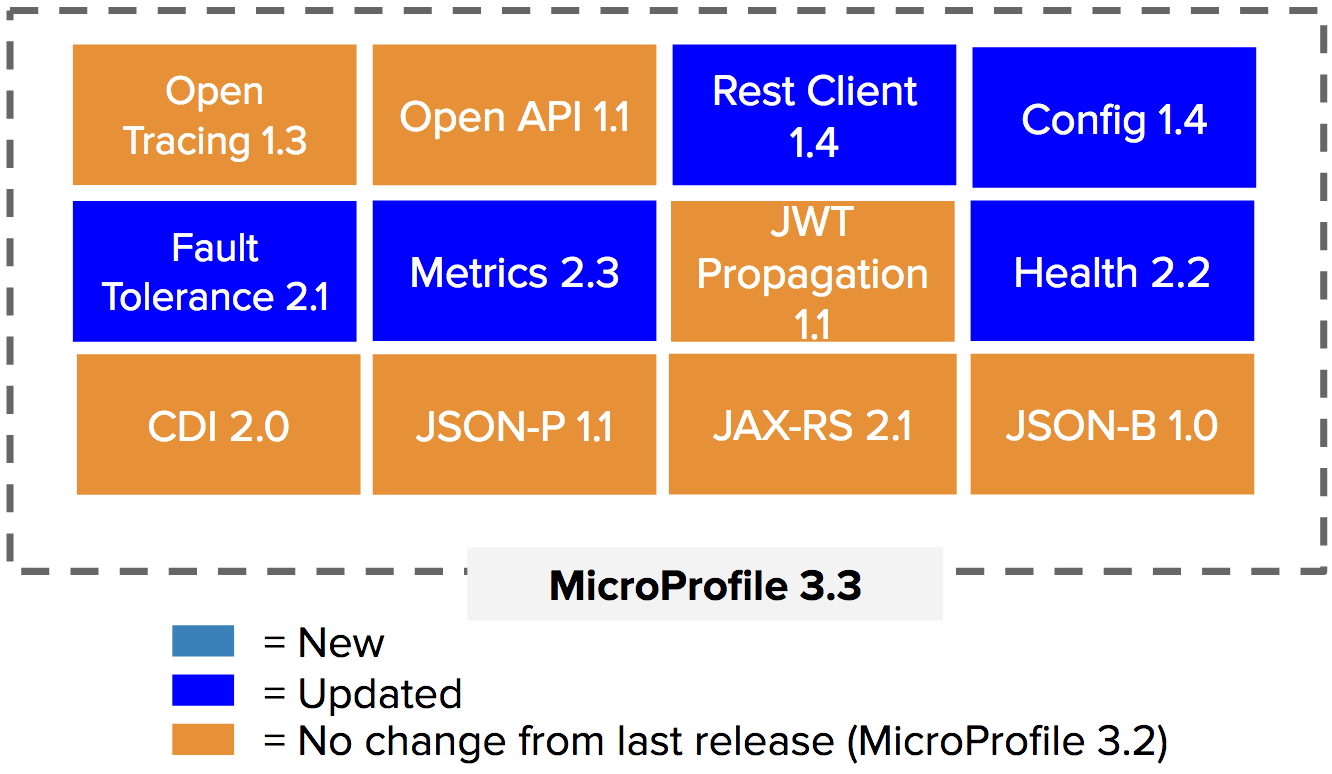
\includegraphics[width=\linewidth]{Images/mp33}
\end{figure}
\end{frame}

\begin{frame}{Eclipse MicroProfile}
\small
    \begin{columns}
        \begin{column}{0.5\textwidth}
    	  Bibliotecas
          \begin{enumerate}
              \item SmallRye
              \item Apache Geronimo
              \item Fujitsu Launcher
          \end{enumerate}
    	\end{column}
    	\begin{column}{0.5\textwidth}  %%<--- here
        JEAS - FatJar, UberJar
    		\begin{enumerate}
                \item DropWizard
                \item KumuluzEE
                \item Helidon (Oracle)
                \item WebSphere/Open Liberty (IBM)
                \item Quarkus (Red Hat)
                \item Payara Micro
                \item Apache TomEE
            \end{enumerate}

    	\end{column}
    \end{columns}
\end{frame}

\begin{frame}{Eclipse MicroProfile}
\small
    \begin{columns}
        \begin{column}{0.5\textwidth}
    	  Micro server
          \begin{enumerate}
              \item Payara Micro
              \item Apache TomEE
          \end{enumerate}
    	\end{column}
    	\begin{column}{0.5\textwidth}  %%<--- here
        Full server (Jakarta EE/Java EE)
    		\begin{enumerate}
                \item Payara
                \item JBoss / Wildfly
                \item WebSphere/Open Liberty
                \item Apache TomEE
            \end{enumerate}

    	\end{column}
    \end{columns}
\end{frame}

\begin{frame}{Eclipse MicroProfile para "modular monolith"}

\begin{columns}
\begin{column}{0.5\textwidth}
	\begin{figure}
		\centering
		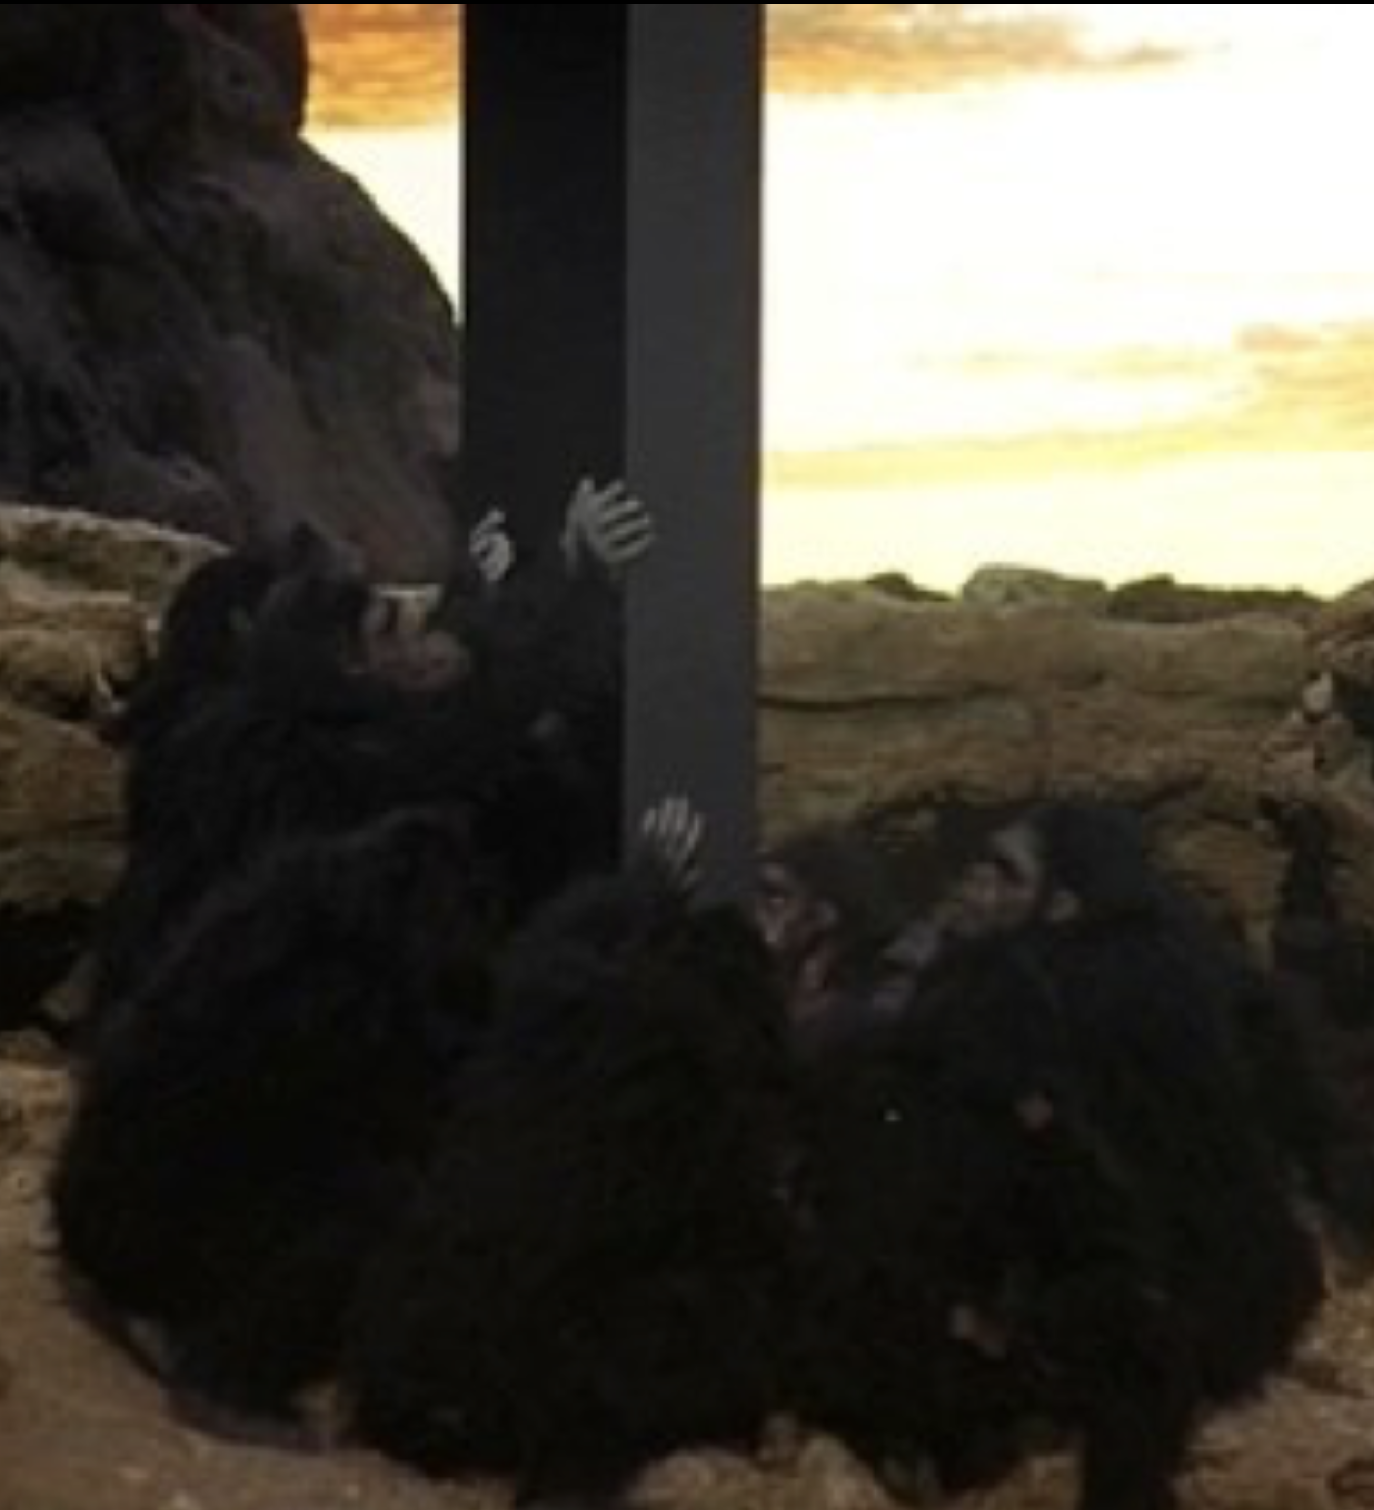
\includegraphics[width=0.7\linewidth]{Images/space}
	\end{figure}
	\end{column}
	\begin{column}{0.5\textwidth}  %%<--- here
		\begin{itemize}
        	\item Integração = CDI
            \item APIs Micro em servers tradicionais
            \item Aproveitar os princípios de arquitetura micro em entornos tradicionais
        \end{itemize}


	\end{column}
\end{columns}
\end{frame}

\begin{frame}{Eclipse MicroProfile para "modular monolith"}

Use cases comuns

\begin{itemize}
    \item Externalização da configuração (módulos intercambiáveis)
    \item Documentação de APIs para integradores e clientes (contratos e interfaces)
    \item Criação de comunicação Typesafe entre módulos via HTTP-Rest (contratos e interfaces)
    \item Tolerância à falhas sem complicações (funcionalidade autônoma)
    \item Gestão de métricas e observabilidade (funcionalidade autônoma)
\end{itemize}
\end{frame}


\section{MP Use cases}

\begin{frame}{Configuração}

\begin{columns}
    \begin{column}{0.7\textwidth}
    	\begin{itemize}
            \item MP Config
            \item Alternativas: Apache Tamaya, DeltaSpike Config
            \item Bom para: Docker, K8s, Maven Profiles + Filtering
            \item Monólito: Configuração no deployment, alternativa simples ao JNDI, evita a necessidade de recompilação
        \end{itemize}
	\end{column}
	\begin{column}{0.4\textwidth}  %%<--- here
        \begin{figure}
        	\centering
        	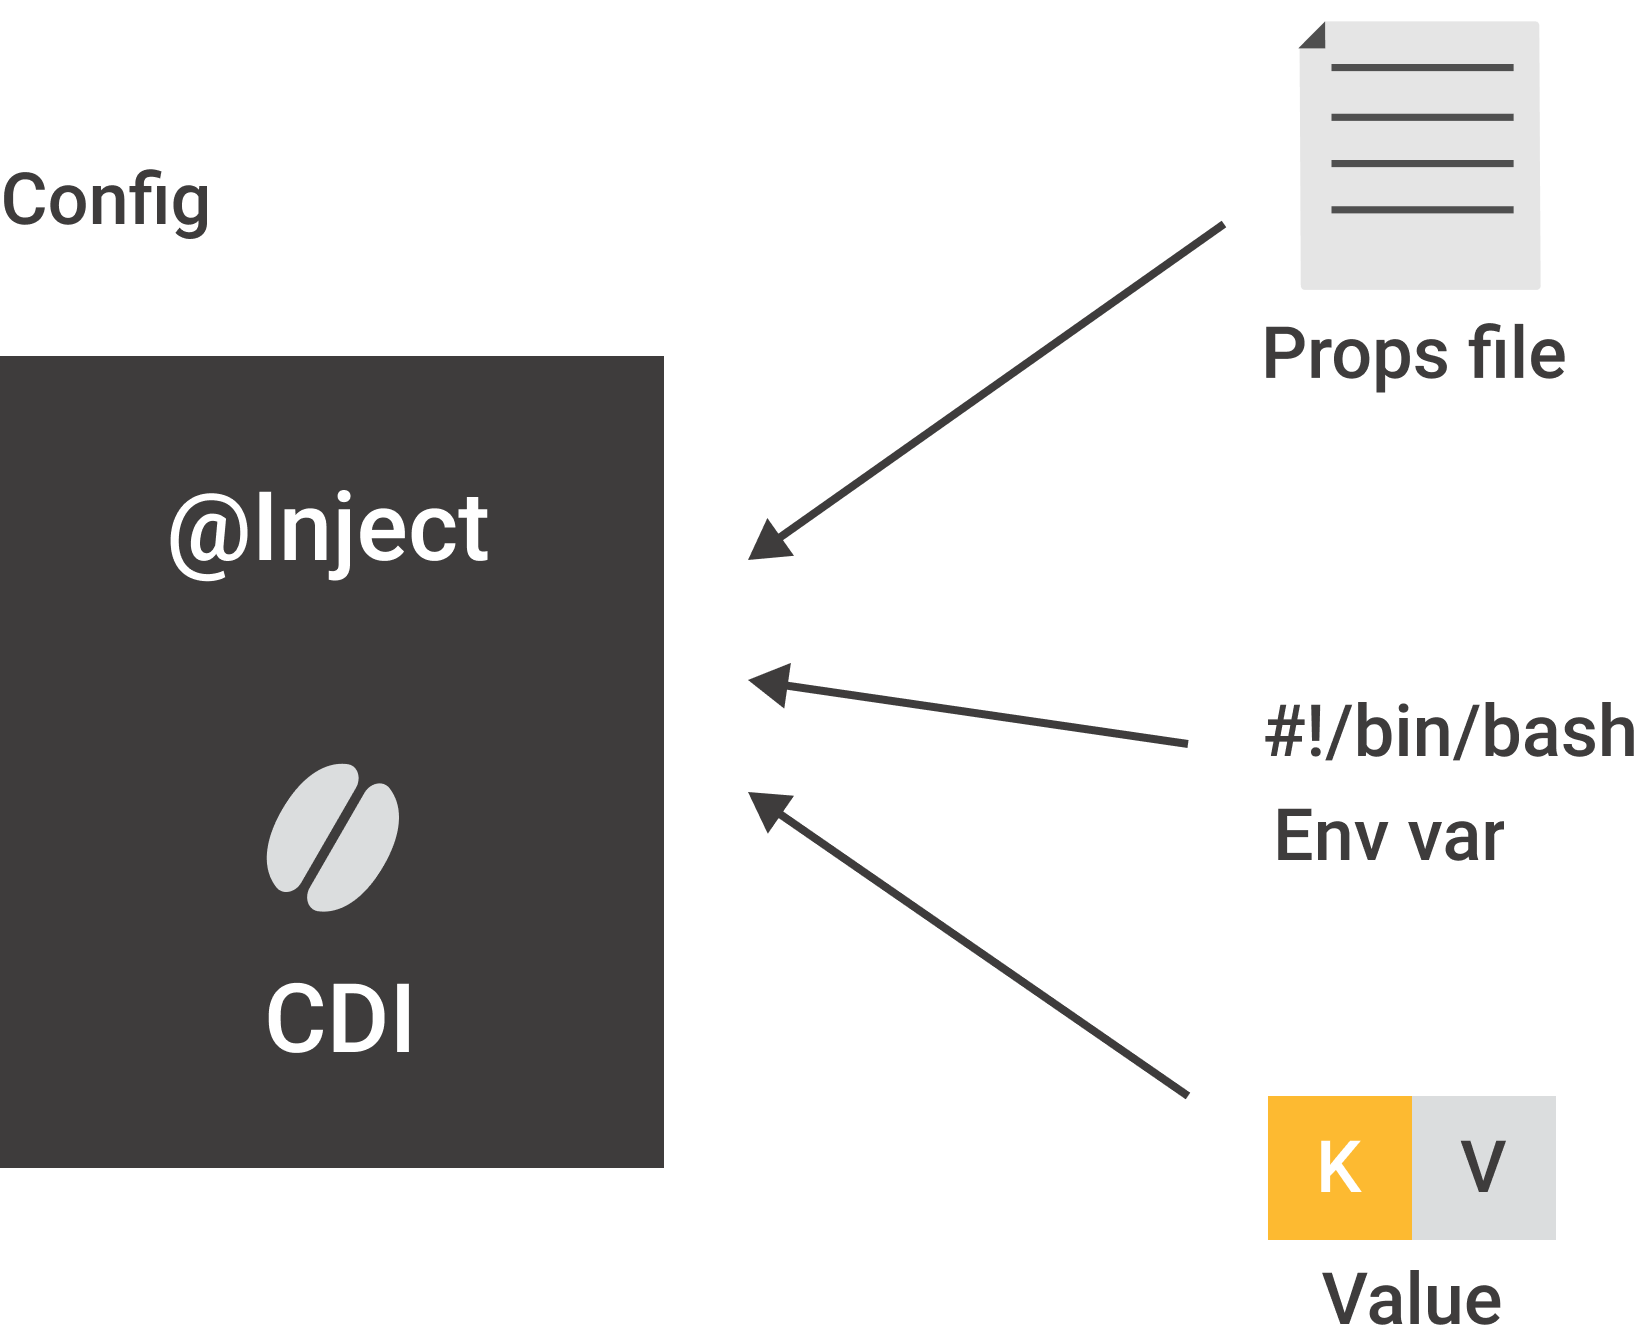
\includegraphics[width=\linewidth]{Images/config}
        \end{figure}

	\end{column}
\end{columns}


\end{frame}

\begin{frame}{Documentação}

\begin{itemize}
    \item MP OpenAPI
    \item Alternativas: Swagger Java
    \item Bom para: Documentação REST
    \item Monólito: Definição de integrações, documentações on-line
\end{itemize}
\end{frame}

\begin{frame}{Comunicação REST TypeSafe}

\begin{columns}
    \begin{column}{0.7\textwidth}
\begin{itemize}
    \item MP TypeSafe REST Client
    \item Alternativas: Jersey, Hoodie
    \item Bom para: Integrações via HTTP
    \item Monólito: Separação de responsabilidade, eventual possibilidade de levar os módulos para microserviçõs
\end{itemize}
	\end{column}
	\begin{column}{0.4\textwidth}  %%<--- here

\begin{figure}
	\centering
	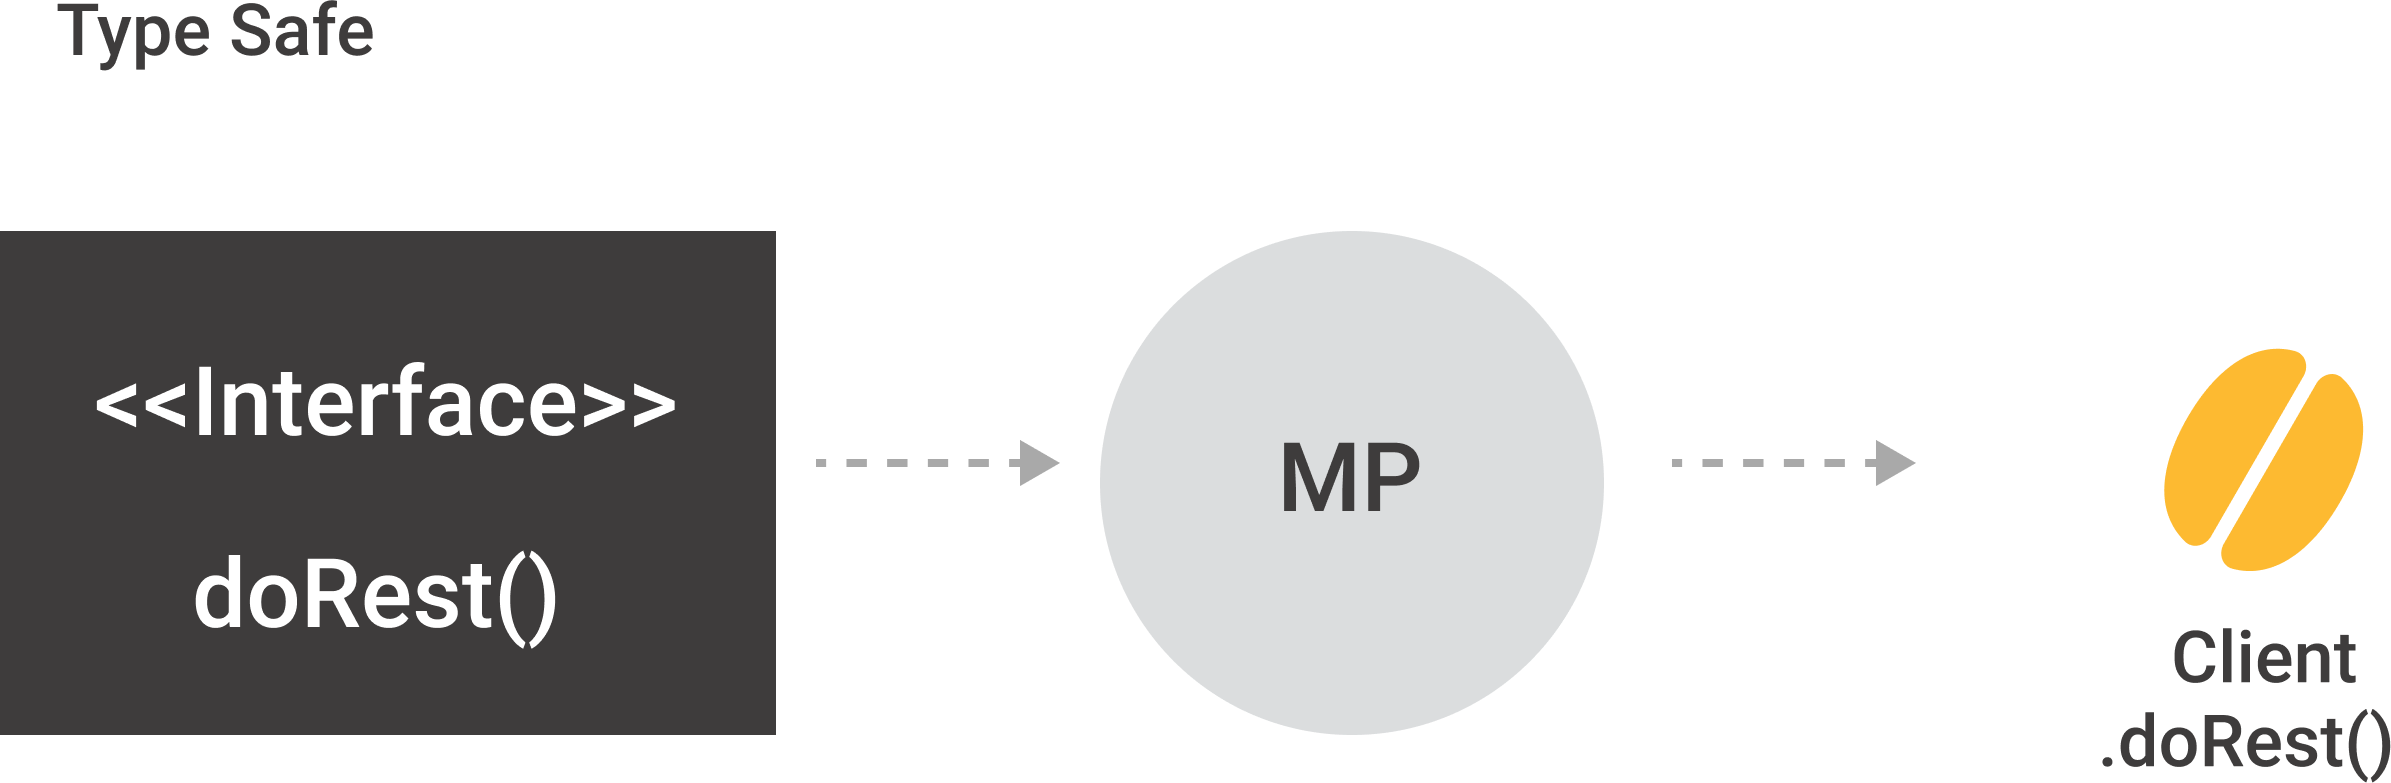
\includegraphics[width=\linewidth]{Images/typesafe}
\end{figure}

	\end{column}
\end{columns}

\end{frame}


\begin{frame}{Tolerância â falhas}

\begin{columns}
    \begin{column}{0.7\textwidth}
\begin{itemize}
    \item MP Fault Tolerance
    \item Alternativas: Hystrix, ResilenceJ
    \item Bom para: Cotas, SLAs, Tolerância à falhas
    \item Monólito: APIs mais resilientes, independência na cadeia de confiança entre serviços
\end{itemize}
	\end{column}
	\begin{column}{0.4\textwidth}  %%<--- here

\begin{figure}
	\centering
	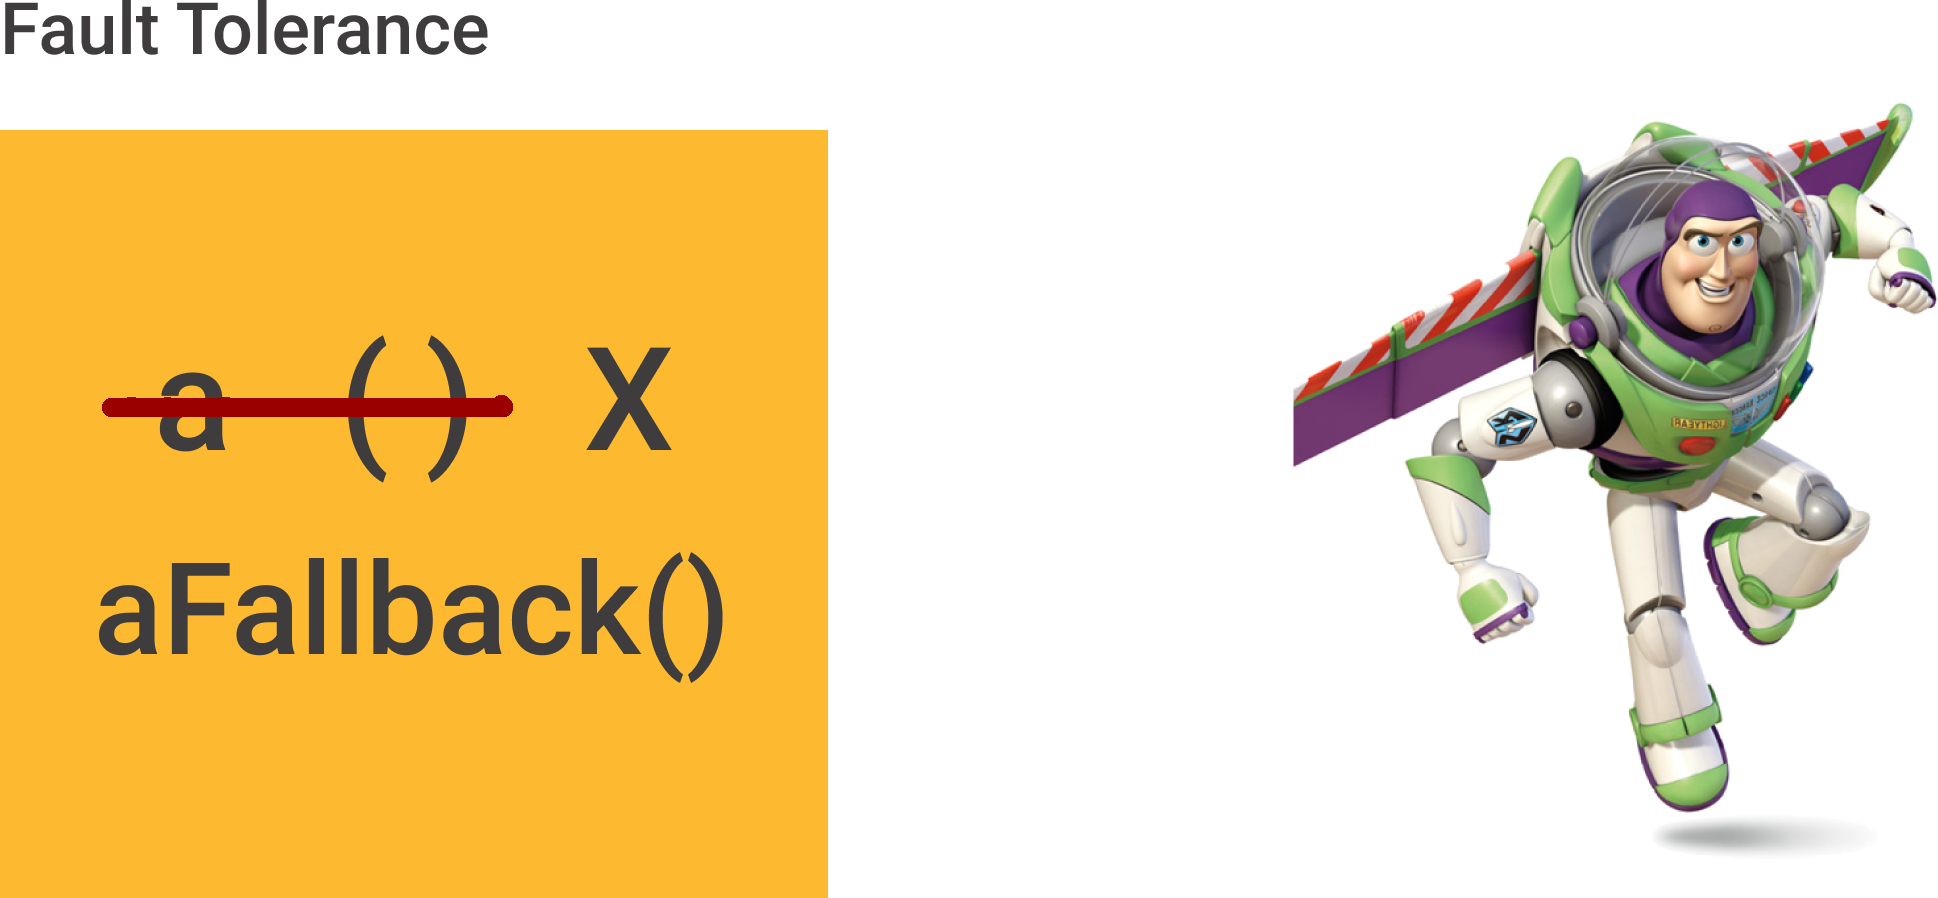
\includegraphics[width=\linewidth]{Images/faulttolerance}
\end{figure}

	\end{column}
\end{columns}

\end{frame}


\begin{frame}{Métricas}

\begin{columns}
    \begin{column}{0.7\textwidth}
\begin{itemize}
    \item MP Metrics
    \item Alternativas: Metrics CDI
    \item Bom para: Docker, K8s
    \item Monólito: Evitar complexidade do JMX, MBeans, monitoramento via http
\end{itemize}
	\end{column}
	\begin{column}{0.4\textwidth}  %%<--- here

\begin{figure}
	\centering
	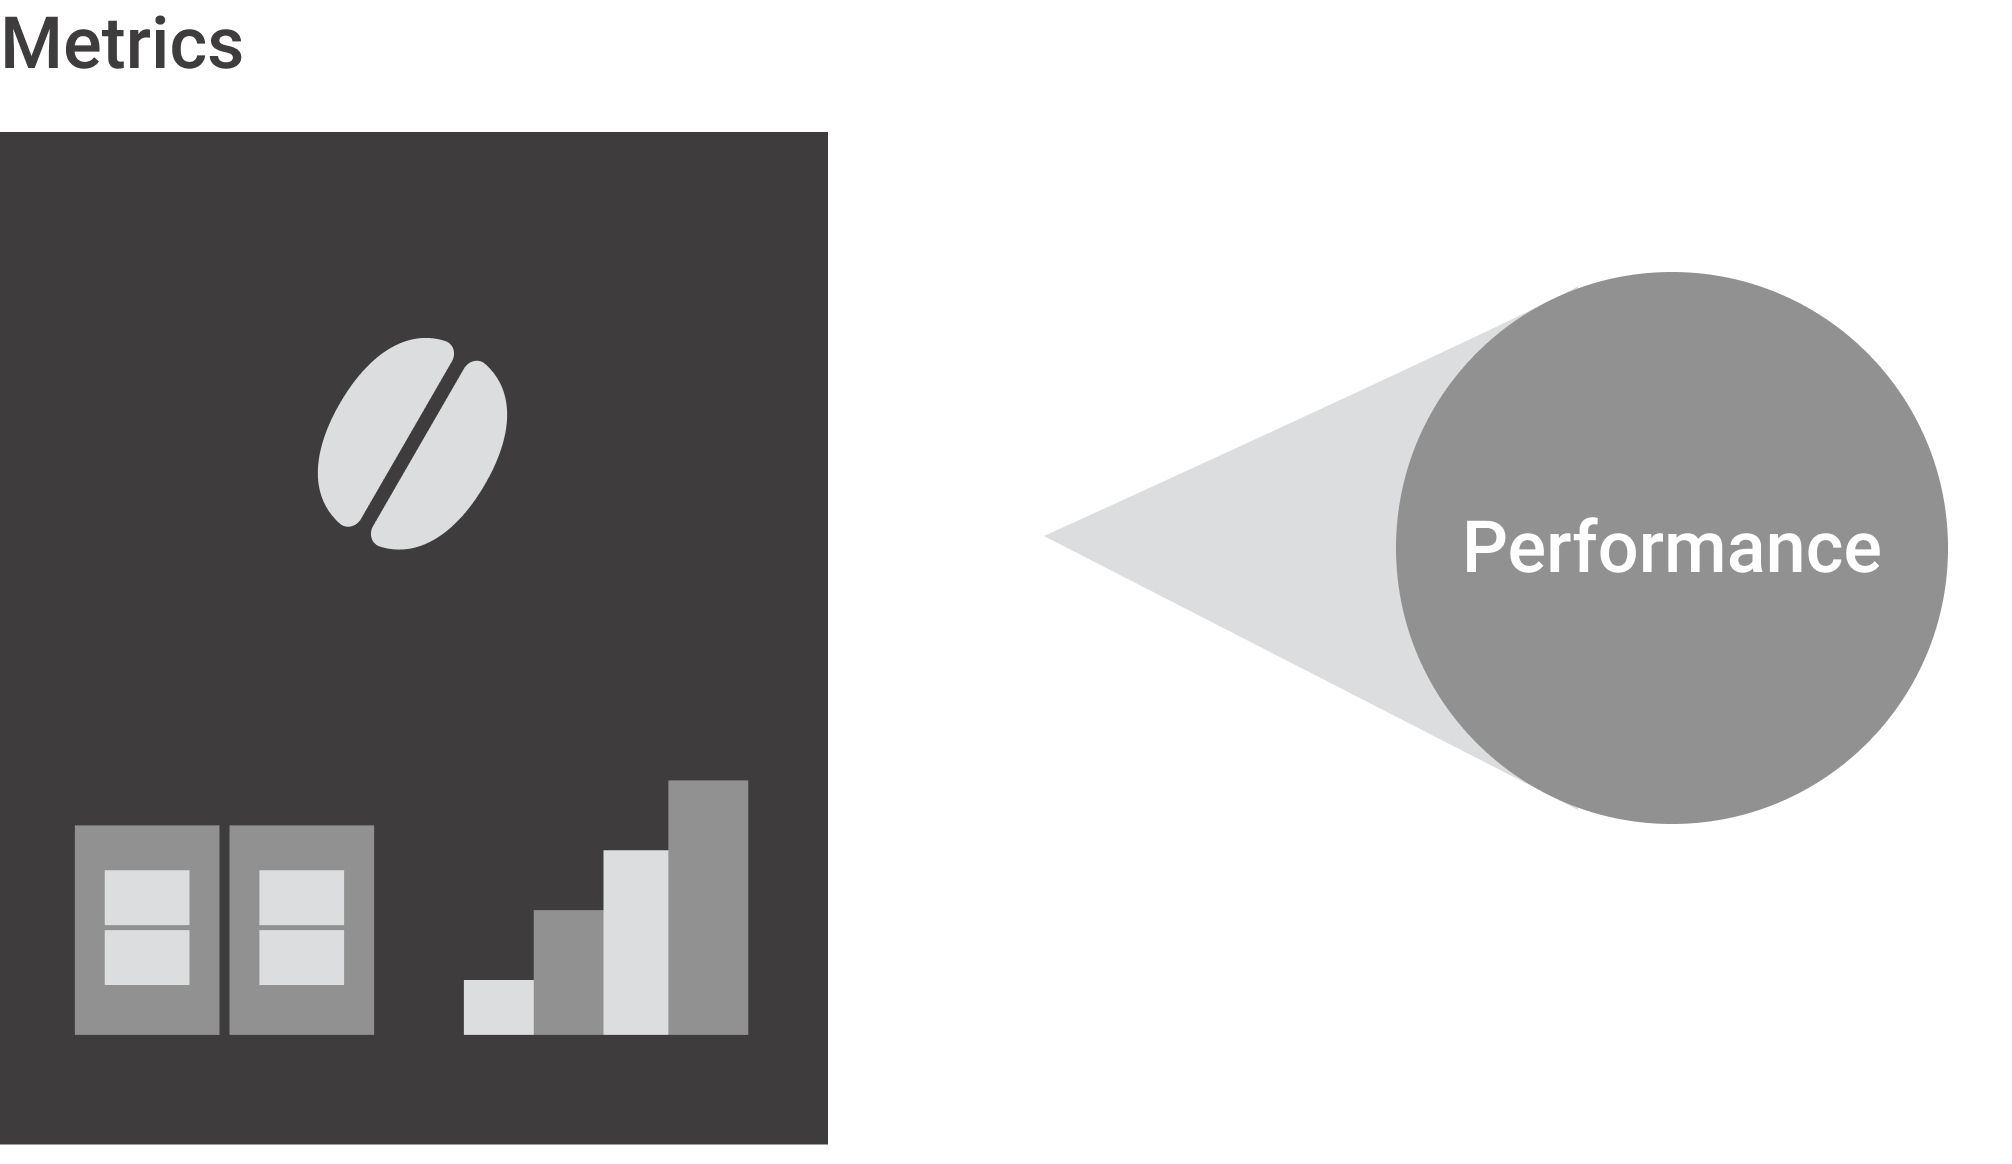
\includegraphics[width=\linewidth]{Images/metrics}
\end{figure}

	\end{column}
\end{columns}

\end{frame}



\begin{frame}{Demo time!}

\begin{itemize}
    \item Payara
    \item Docker
    \item Oracle cloud
\end{itemize}

Objetivo: Olá mundo, modular, autônomo e intercambiável

Java 11, JAX-RS, CDI, MicroProfile

\normalsize  \url{https://github.com/tuxtor/MP-Workshop}\\

\end{frame}




\begin{frame}{Víctor Orozco}
\begin{columns}[T] % contents are top vertically aligned

	\begin{column}[T]{4cm} % alternative top-align that's better for graphics
		\begin{figure}
			\centering
			
\includegraphics[width=\linewidth]{Images/logos}
		\end{figure}
	\end{column}
	\begin{column}[T]{6cm} % each column can also be its own environment
		\begin{itemize}
			\item me@vorozco.com
			\item \href{https://twitter.com/tuxtor}{@tuxtor}
			\item \href{http://vorozco.com}{http://vorozco.com}
			\item \href{http://tuxtor.shekalug.org}{http://tuxtor.shekalug.org}
		\end{itemize}
	\begin{center}
		
\includegraphics[width=0.1\linewidth]{Images/cclogo}
		\\
		This work is licensed under a Creative Commons Attribution-ShareAlike 3.0.
	\end{center}
	\end{column}
\end{columns}
\end{frame}


\end{document}

